\documentclass[]{report}
\usepackage{SourceSerifPro}

% Overwrite \begin{figure}[htbp] with \begin{figure}[H]
\usepackage{float}
\let\origfigure=\figure
\let\endorigfigure=\endfigure
\renewenvironment{figure}[1][]{%
\origfigure[b]
}{%
\endorigfigure
}

% fix for pandoc 1.14
\providecommand{\tightlist}{%
  \setlength{\itemsep}{0pt}\setlength{\parskip}{0pt}}

% TP: hack to truncate list of figures/tables.
\usepackage{truncate}
\usepackage{caption}
\usepackage{tocloft}
% TP: end hack

\usepackage{setspace}
\setstretch{1.15}
\usepackage{amssymb,amsmath}
\usepackage{ifxetex,ifluatex}
\usepackage{fixltx2e} % provides \textsubscript
\ifnum 0\ifxetex 1\fi\ifluatex 1\fi=0 % if pdftex
  \usepackage[T1]{fontenc}
  \usepackage[utf8]{inputenc}
\else % if luatex or xelatex
  \ifxetex
    \usepackage{mathspec}
    \usepackage{xltxtra,xunicode}
  \else
    \usepackage{fontspec}
  \fi
  \defaultfontfeatures{Mapping=tex-text,Scale=MatchLowercase}
  \newcommand{\euro}{€}

    \setmainfont{SourceSerifPro}
    \setsansfont{SourceSansPro}
\fi
% use upquote if available, for straight quotes in verbatim environments
\IfFileExists{upquote.sty}{\usepackage{upquote}}{}
% use microtype if available
\IfFileExists{microtype.sty}{%
\usepackage{microtype}
\UseMicrotypeSet[protrusion]{basicmath} % disable protrusion for tt fonts
}{}
\usepackage{longtable,booktabs}
\usepackage{graphicx}
\makeatletter
\def\maxwidth{\ifdim\Gin@nat@width>\linewidth\linewidth\else\Gin@nat@width\fi}
\def\maxheight{\ifdim\Gin@nat@height>\textheight\textheight\else\Gin@nat@height\fi}
\makeatother
% Scale images if necessary, so that they will not overflow the page
% margins by default, and it is still possible to overwrite the defaults
% using explicit options in \includegraphics[width, height, ...]{}
\setkeys{Gin}{width=\maxwidth,height=\maxheight,keepaspectratio}
\ifxetex
  \usepackage[setpagesize=false, % page size defined by xetex
              unicode=false, % unicode breaks when used with xetex
              xetex]{hyperref}
\else
  \usepackage[unicode=true]{hyperref}
\fi
\hypersetup{breaklinks=true,
            bookmarks=true,
            pdfauthor={},
            pdftitle={},
            colorlinks=true,
            citecolor=blue,
            urlcolor=blue,
            linkcolor=magenta,
            pdfborder={0 0 0}}
\urlstyle{same}  % don't use monospace font for urls
\setlength{\parindent}{0pt}
\setlength{\parskip}{6pt plus 2pt minus 1pt}
\setlength{\emergencystretch}{3em}  % prevent overfull lines
\setcounter{secnumdepth}{0}

\date{}
\usepackage{ragged2e}
\usepackage{biblatex}
\usepackage{graphicx}
\usepackage{pdflscape}
\addbibresource{}
\RaggedRight

\usepackage{fancyhdr}
\pagestyle{fancy}
\fancyhead{}
\fancyfoot{}
\newcommand{\ssp}{%
  \fontfamily{phv}\fontsize{9}{11}\selectfont}

\lhead{\ssp \leftmark}
\rhead{\ssp \thepage}
\lfoot{\ssp \leftmark}
\rfoot{\ssp \thepage}
\renewcommand{\footrulewidth}{0.7pt}

\usepackage{rotating}
\usepackage{longtable,booktabs}

\begin{document}

{
\hypersetup{linkcolor=black}
\setcounter{tocdepth}{2}
\tableofcontents
}

\chapter*{Abstract}\label{abstract}
\addcontentsline{toc}{chapter}{Abstract}

The minimum set of genes of an organism refers to the smallest set of
genes that can support a free living organism. In this study the minimum
set of genes was described using three machine learning models are used
(Naive Bayes Classifier, Random Forest Classifier, and Artificial Neural
Network), each trained with data annotated using the COG (Clusters of
Orthologous Groups) framework. The models show promising predictive
power (Naive Bayes Classifier=0.80, Random Forest Classifier=0.78, and
Artificial Neural Network=0.87). Each model is then subjected to feature
extraction to describe a its own interpretation of the minimum set of
genes. Each of the models' set of genes are compared the CEG databases
set of essential genes. The results show that even though the Naive
Bayes Classifier does not have the most predictive power, it is able to
perform best in the set comparisons between the CEG database. In
particular it was the best model in classifying which genes are
non-essential (Jaccard index of 0.0058 when compared to CEG set of
nonessential genes). These findings show that machine learning
algorithms can provide good modelling tools for the minimum set of
genes. The methods discussed in this paper can be applied to improve our
understanding of the concepts behind gene essentiality and the
requirements of creating life.

\chapter{Introduction}\label{introduction}

The first free living genome was sequenced in 1995 (R. Fleischmann et
al., 1995). It was the genome of the bacterium \emph{H. influenzae},
containing 1,830,137 base pairs. Eight years after the publishing of
\emph{H. influenzae} genome, in 2002, the Human Genome Project was
completed (Tripp \& Grueber, 2011). Started in 1990, the project was a
product of contributions from multiple universities and laboratories
around the world. The project involved a laborious process of
experimentally obtaining segments of DNA and a more laborious process of
reassembling the segments. After 12 years, the whole project completely
sequenced the 3.3 billion base pair long human genome. The Human Genome
Project inspired the emergence of research about genomes and sequencing
tools and processes. The project also inspired the emergence of many
genomics related researches in the field of bioinformatics, like
sequence analysis, genome annotation and sequence databases.

\section{There is an abundance of genomic
data}\label{there-is-an-abundance-of-genomic-data}

Currently, the field genomics is on the background of the big data and
machine learning age. The emergence of big data and the advancements in
bio-informatics brought upon the abundance of high quality genetic data
(Mushegian \& Koonin, 1996; Thanassi, 2002; Tonder et al., 2014). This
is facilitated by public databases like GenBank, the Sequence Read
Archive and European Nucleotide Archive (ENA) (Benson et al., 2000;
Leinonen et al., 2011; Leinonen, Sugawara, \& Shumway, 2011). These
databases store sequences derived from innovations from next generation
sequencing. Next generation sequencing is a group of modern genome
sequencing technologies that are reportedly powerful enough to sequence
the whole human genome in a single day. Computationally powerful
machines combined with computationally powerful techniques like next
generation sequencing, give the field of genomics better tools as it
revisits some of biology's difficult questions.

\section{The fewest parts to construct a
cell.}\label{the-fewest-parts-to-construct-a-cell.}

One of difficult open questions in biology right now is the study on the
search for the minimal set of genes. Finding the minimal gene set is the
attempt to identify the smallest set of genes that can support life
({\textbf{???}}). There have been many attempts to answer this question
through theory and small scale experimentation (Glass et al., 2006).
Identifying minimal gene set can provide basis for synthetic biology
(Lluch-Senar et al., 2015), which is an emerging interdisciplinary field
of biology and engineering. This field studies the synthesis and
application of artificial biological systems. Although there are many
attempts in creating artificial life that are relatively successful,
none of these attempts have gone as close as creating free living cells
(Ferber, 2004). By finding the minimal set of genes that can support
life the current understanding of simple biological systems will improve
making the road to the first free living artificial life one step
closer.

\section{Effective ways to kill
cells}\label{effective-ways-to-kill-cells}

Another application of determining the minimal set of genes is in
differentiating essential and non-essential genes in bacterial genomes.
This will give antibiotics better techniques in killing pathogenic
bacteria by disabling essential genes (Akerley et al., 1998). Gene
targeting with the knowledge of gene essentiality can be a very
effective means of killing pathogenic bacteria (R. Zhang \& Lin, 2009).
Knowledge of gene essentiality will provide pharmaceutical research
advanced antibiotic techniques like general bacteria killers and species
specific bacteria killers.

\section{The goals of this study}\label{the-goals-of-this-study}

This study aims to model the minimum set of genes using machine learning
algorithms. This study also aims to document the applicability of
machine learning methods as modelling tools for the minimum set of
genes. The ultimate goal of this study is to contribute to the
understanding of the minimum set of genes by proposing its methodology.

In the following chapter this study will discuss, the biological
concepts relating to the minimal set of genes. The following chapter
will also contain previous work that contribute to the study on the
minimal set of genes along with the accomplished milestones and gaps in
knowledge. The next chapter will discuss on which methods this study has
chosen to contribute to the current gaps in knowledge. After that there
will be a chapter comparing the results between the findings from this
and the findings from previous studies. Finally, the last chapter will
include a summary of the whole paper, some recommendations and the
impact of this study.

\chapter{Related Work}\label{related-work}

\section{Theoretical Perspectives}\label{theoretical-perspectives}

\subsection{Genes, Proteins and Function
Expressions}\label{genes-proteins-and-function-expressions}

The central dogma of molecular biology explains the how genetic
information flows within a biological system (Crick, 1958). This idea
was first stated by one of the co-discoverers the structure of a the
DNA, Francis Crick. The most simplistic description of the central dogma
states that ``DNA makes RNA and RNA makes protein'' (Leavitt, 2010). The
dogma is a framework that describes three general processes of
biological sequential information transfers.

\subsubsection{Replication}\label{replication}

DNA replication is simply the processes that facilitate the reproduction
of DNA sequences. This process is essential since DNA information must
be reproduced when the cell itself reproduces (Leavitt, 2010).

\subsubsection{Transcription}\label{transcription}

This is the process in which DNA information in a particular section is
replicated into another type of biological sequence information, the
RNA. There many biological process that facilitate the transcription of
DNA to RNA but RNA is basically a copy of the information found in the
DNA. RNA serves as a middle man/messenger sequence between DNA and
protein sequences. This extra middle step is essential in the whole
process as it protects the information located in the DNA. Instead of
subjecting DNA to the dangers of the process of translation, the RNA
copy is used instead (Leavitt, 2010).

\subsubsection{Translation}\label{translation}

This process takes place after an RNA is transcripted from DNA. An RNA
makes its way to a ribosome, a cellular organelle that facilitates
translation. Using multiple enzymatic processes within the ribosome, RNA
sequences of nucleoases (A,U,G,C) are translated into protein sequences
of amino acids. Every three nucleobases in the RNA has a corresponding
translation to one of the 20 amino acids. Starting from RNA, the
translation process yields a protein sequence of amino acids. These
proteins are responsible for various biological functions that are
expressed in organisms (Leavitt, 2010).

\subsection{Essential and Non-essential
Genes}\label{essential-and-non-essential-genes}

Genes range from as few as 480 base pairs ,as shown by the bacterium
\emph{Mycoplasma genitalium}, to 100,000 to 150,000, as shown by
multi-cellular eukaryotes like humans (E. V. Koonin, 2000). Not all of
these genes are completely essential for the survival of an organism.
Some of these genes are functionally redundant. Functionally redundant
genes are two or more genes that share the same function when expressed.
This means that only one of these genes is needed for surviva. (E. V.
Koonin, 2000; Nowak, Boerlijst, Cooke, \& Maynard Smith, 1997). The
concept of essential genes refer to the smallest set of genes which
produces a fully functioning organism under the best conditions of
living, that is, nutrients are abundant and stress is absent (E. V.
Koonin, 2000). Researchers have considered the upper bound of the
minimum set of genes to be 480 genes. This number is chosen as it is the
number of genes of the bacterium \emph{Mycoplasma genitalium}. \emph{M.
genitalium} is the organism with the smallest known genome (C. M. Fraser
et al., 1995 ).

\subsection{Core genome}\label{core-genome}

One of the approaches for the determination of the minimal set of genes
uses the concept of the core genome. The core genome of a group of
organisms refer to the set of genes shared by all organisms under said
group of organisms. This set of genes doesn't include genes that vary
for other organisms in the same group (genes that only contribute to the
diversity of said group of organisms) (Tettelin et al., 2005; Tettelin,
Riley, Cattuto, \& Medini, 2008 ). Since the core genome of a group of
organisms consists of genes shared by multiple genomes, said core genome
could be a good candidate for the minimal gene set.

\section{State of the Art}\label{state-of-the-art}

\subsection{\texorpdfstring{Using the \emph{Mycoplasma genitalium}
bacteria}{Using the Mycoplasma genitalium bacteria}}\label{using-the-mycoplasma-genitalium-bacteria}

For many researchers, \emph{Mycoplasma genitalium's} genome has been the
primary candidate for the core bacterial gene set. It is widely accepted
that the length of this bacterium's gene set is the upper bound for the
bacterial genome (C. M. Fraser et al., 1995). Global transposon
mutagenesis on \emph{M. genitalium} is a well studied approach on the
study of the minimal gene set.

Trasposon mutagenesis is a process that allows gene segments to be
transferred to another organism. Because of the insertion of the
introduced gene during transposon, the host organism (the owner of the
interupted gene) experiences a mutation. By deliberately interrupting
the host's chromosomes, researchers can infer information on the
function of the hosts genes (L. Hamer, DeZwaan, Montenegro-Chamorro,
Frank, \& Hamer, 2001). Hutchison III et. al. (1996) used transposon
mutagenesis on \emph{M. genitalium's} genome along with its closest
relative \emph{M. pneumoniae} to identify which gene locations are
essential and which are nonessential (Hutchison III, 1999). The
researchers did this by deliberately inserting extant genes to introduce
mutations to \emph{M. genitalium} and \emph{M. pneumoniae} and studying
the effects of these mutations to their survivability (1999). Their
analysis suggests that 265 to 350 of the 480 protein-coding genes of
\emph{M. genitalium} are considered essential.

\emph{M. genitalium's} gene sequence has also been used in the
comparative genomics approach of the search for the minimal bacterial
gene set. Using protein sequence analysis, a bioinformatics approach of
comparing sequences described by Koonin (1996), Musheigian and Koonin
(1996) compared \emph{M. genitalium} with \emph{Haemophilus influenzae}
and found 240 orthologs (genes with the same functions but not
necessarily same sequences) (1996 ). This means that the two bacteria
share a set of 256 gene functions. Genes outside of the 256 orthologs
can be considered non-essential genes since either bacterium can survive
without them.

\subsection{Experimentally determined essential
genes}\label{experimentally-determined-essential-genes}

DEG 5.0 is a database of genes where their essentiality to survival is
experimentally determined (R. Zhang \& Lin, 2009 ). This database is an
improved version of DEG 1.0, created 5 years. It contains information
about the essential genes, the experimental method used to determine
their essentiality, and their associated references. The most common
experimental methods of confirming gene essentiality are direct gene
deletions or random mutagenesis (R. Zhang \& Lin, 2009 ).

\paragraph{Direct deletions}\label{direct-deletions}

Mori et. al. (2015) identified 328 essential gene candidates for the
bacterium \emph{Escherichia coli} using direct gene deletions (2015).
Their method involves experimentally ``knocking out'' gene segments and
studying the effect of the gene's abscence to the survivability of
\emph{E. coli}. Kobayashi et. al. (2003) and de Berardinis et. al.
(2008) also used single gene deletions to determine essential genes for
\emph{Bacillus subtilis} and \emph{Acinetobacter baylyi} respectively
(2008; 2003).

\paragraph{Transposon mutagenesis}\label{transposon-mutagenesis}

Transposon mutagenesis, just as discussed previously, is an approach
using transposons which insert in extant genes in random positions in
the genome. At publication of Zhang's (2009) paper, 7 prokaryote
genomes' essential genes were studied.The number of essential genes for
each specific prokaryote ranges between 300-650 (R. Zhang \& Lin, 2009).

\subsection{Use of machine learning and statistical
methods}\label{use-of-machine-learning-and-statistical-methods}

The current trend of research in this study is starting to shift from
experimental methods to qualitative analyses due to the emergence of
statistical and machine learning tools. Van Tonder et. al. (2014) used
this approach to determine bacterial core genomes to specific
populations (Tonder et al., 2014 ). The researchers developed Bayesian
decision models to estimate the number of core genes for each
population. The researchers built the Bayesian prior of the model using
the probabilities of gene occurrences as posterior. Said Bayesian prior
rule is then used to determine if a gene is present in the core genes.

\subsection{Clusters of Orthologous Groups
(COGs)}\label{clusters-of-orthologous-groups-cogs}

Koonin started his work on the minimum set of genes in 1996 with
Musheigan in a time when completely sequenced genomes were scarce. In
fact it was only 1995 when the first bacteral genome (\emph{H.
influenzae}) was completely sequnced. During this time he was able to
suggest the first iterations of the minimum gene set concept by
comparing two relatively distant bacteria (\emph{M. genitalium} and
\emph{H. influenzae}) (Mushegian \& Koonin, 1996 ). A year later Koonin,
along with Tatusova and Lipman (1997) proposed a new perspective in
protein classification (1997). This was the first conceptions of
Cluster's of Orthologous Genes (COG). The study created families of gene
encoded proteins according to their orthology (having same functions).
At the time of the study's publishing, 720 COG's were identified, each
with individual orthologous proteins or orthologous set of proteins. The
COG classification was used as a framework to predict gene functions of
poorly sequenced genome. Using this new COG tool in hand, in the year
2000, Koonin revisited the minimal gene set concept (E. V. Koonin, 2000
). The COG approach along with more sequenced genomes, allowed Koonin to
compare more genes. Koonin found a smaller set of conserved gene
functions (about 30\% of the 1996 minimum gene set size) across 25
sequenced genomes which oppose his previous finding in 1996.

\section{Gaps in knowledge}\label{gaps-in-knowledge}

\subsection{Comparative methods fail on highly diverse group of
organisms}\label{comparative-methods-fail-on-highly-diverse-group-of-organisms}

The most common methods of comparative genomics usually involve studying
the intersection of gene sets. Examples of this approach are Koonin and
Musheigian's (1996) comparison between *M. genitalium** and \emph{H.
influenzae} and Tettelin et. al's (2005) \emph{Streptococcus agalactiae}
pangenome (1996; 2005 ). This approach worked very well on these papers
because these studies involve comparing two closely related genes or
comparing a group of genes belonging in a population of organisms. A
problem arises when the collection of genes compared is in a diverse
group. The intersection of gene sets on a collection of diverse group
will yield a very small set (Tonder et al., 2014). The reason for this
limitation is because the conservativeness of this comparative approach
fails to take into account the complex relationships of genes and
metabolic functions like synthetic lethality (e.g.~genes A and B are
only lethal if both are present in the same genome) (Mori et al., 2015;
Pál et al., 2006) and conditionally essential genes (e.g.~gene A is
essential given C) (Gerdes et al., 2006).

\subsection{Bacteria's resilience to transposon mutagenesis' disruption
and single gene
deletions}\label{bacterias-resilience-to-transposon-mutagenesis-disruption-and-single-gene-deletions}

Hutchison (1999) discussed some of the limitations of transposon
mutagenesis in his paper. Hutchison's paper reported unexpectedly low
results of 12 essential genes out of 1354 (less than 1\%). According to
his discussion this may be because his experiment failed to disrupt some
of the genes providing incorrect results. Hutchison also suggests that
erroneous results may be due to some cells keeping a functional
duplicate copy of the otherwise disrupted gene.

\subsection{Previous methodologies don't make use of current state of
the art gene
annotations}\label{previous-methodologies-dont-make-use-of-current-state-of-the-art-gene-annotations}

As discussed in the previous sections, knowledge about the minimum set
of genes evolve as new bioinformatics and genomic tools evolve. As an
example, Koonin's body of work in the concept of minimum set of gene's
has undergone multiple revisions as new tools emerge (E. V. Koonin, 2000
; Mushegian \& Koonin, 1996). Koonin's 2000 meta study on the concept of
the minimum gene set make use of the early version of the COG database
tool (Tatusov, 1997). At the time of the paper's publishing, Koonin
worked with 25 completely sequenced genomes and the COG the database
contained 2112 unique COGs. On the other hand, at the time of this paper
writing the most recent version (2014 update) of the COG database
contains 5665 unique COG's (Galperin, Makarova, Wolf, \& Koonin, 2015).
The emergence of more completely sequenced genomes and better annotation
tools prompt a revisit of the minimum gene set concept. This time around
we have access to robust machine learning techniques to study this
abundant gene data.

\chapter{Research questions}\label{research-questions}

Based on these gaps in knowledge this research question is formulated:

\subsubsection{Are these machine learning classifiers a valid tool for
determining the minimal set of
genes?}\label{are-these-machine-learning-classifiers-a-valid-tool-for-determining-the-minimal-set-of-genes}

Although, there have been few studies that use machine learning tools in
the study of the minimum set of genes, there have been no studies that
document the applicability of various machine learning methods (Tonder
et al., 2014). Basing on these few promising machine learning studies
this study hypothesizes that machine learning classifiers will be a
useful tool to be used in determining the minimal set of genes.

\chapter{Methodology}\label{methodology}

\section{Data Collection}\label{data-collection}

\subsection{Genes as features}\label{genes-as-features}

To find the minimum set of bacteria genes to sustain a valid bacteria, a
machine learning classification model was to be created built on
features based on the genomic data. By building a model that can
recognize valid and free living bacteria, this study can also propose on
what features characterize a valid bacteria. These features used to
build the model should represent genes of said bacteria. By studying on
how the machine learning algorithms built the model we can infer which
genes are the best determinants for characterizing a valid and free
living bacteria and by consequence which genes are required to create a
bacteria. But instead of focusing on the predictive and classification
abilities of the model, the focus of this study was to analyse which
features (genes) are strongest determinants. Of course the
classification model built must also be a competent classifier, but this
is only to ensure that the model built is correct and unbiased.

\subsection{Positive and Negative
data}\label{positive-and-negative-data}

The data used in this study are genes with functions annotated according
to COG's (cluster of orthologous genes). The data is divided into 2
groups, positive group (valid free living bacteria) and negative group
(unculturable and non free living bacteria). Both sets are comprised of
multiple samples of fully sequenced bacterium preprocessed by the
Philippine Genome Center. Each column in the data (feature) represents a
COG profile. For each instance of bacteria, the values for each cell
represents the frequency of the COG's found in said bacterium's genome.
The model requires a negative set of data so that the models have a way
to differentiate valid bacteria to non valid bacteria. Without the
opposite groups the model built would be unable to make unbiased
generalizations of the the characteristics of the bacterial core genome.

\section{Training and Testing}\label{training-and-testing}

The process for model creation for the three models are identical. The
data is split into two partitions, training and testing. The training
partition is used to fit the model to the data and the testing partition
is used to calculate the model's validation score. It is important that
data is not shared by the two partitions. This rule is kept so that the
model's tests can detect if the classifier is able to generalize on the
data or it merely overfits on the data.

Overfitting occurs when the model describes the data's noise instead of
the underlying relationship of genes and genome validity of bacteria. A
model's overfitting is manifested by having exceptional scores on its
training while having poor scores on its testing. This will happen if
the model is too biased on the training partition and its noise and
specificities instead of generalizing the relationships (M. K. Smith,
2014). The precautions to avoid overfitting is different for each model
and these precautions will be discussed in their own sections later. The
ratio of splitting into partitions should also be an informed choice.
Leaving too little data instances for the training partition will
negatively affect the model's accuracy. While leaving too little data
instances for the testing partition will create unreliable tests. The
two partitions of data must be large enough to be equivalent
representations of each other (Steinberg, 2014).

\section{Model Choices}\label{model-choices}

\subsection{Naive Bayes}\label{naive-bayes}

Naive Bayes is suitable for classifiers with features that represent
frequency or set elements. This applies to the data set used in this
study where frequency is the frequency of a particular COG in a
bacterium's genome. Each data instance can also be represented as a set
of COG's that fully comprises the bacterium's genome (H. Zhang, 2004).

\subsubsection{Model Fitting}\label{model-fitting}

The Naive Bayes family of classifiers are created based on Bayesian
theorem. This algorithm is naive in the sense that it makes a naive
assumption that all of the features in the model are mutually
independent of each other. Applying Bayes theorem in bacterium data
gives this relationship:

\begin{equation} P(y|x_{1},...,x_{n}) = \frac{P(y)P(x_{1},...,x_{n}|y)}{P(x_{1},...,x_{n})}  \end{equation}

Where \(P(y|x_{1},...,x_{n})\) is the posterior probability of a
bacterium being valid or invalid (\(y\)) given that the probabilities of
gene occurences (\(x_i\)) are \(x_{1},...,x_{n}|y\) (H. Zhang, 2004).

\(P(y)\) refers to the prior probability, or the general probability of
the occurences of valid and invalid bacteria. There are no papers that
describe the actual probability distribution of valid and invalid
bacterium in the wild therefore the value used for the prior probability
is the probability distribution of the data provided.
\(P(x_{1},...,x_{n}|y)\) refers to the likelihood probability or the
likelihood of gene occurences to be \(x_{1},...,x_{n}\) for each type of
data (\(y\), valid or invalid bacteria). The values \(x_{1},...,x_{n}\)
are frequency distributions of each gene (n=4347) in a given bacterium
over the total number of gene occurrences in the whole dataset.

Naive Bayes family of classifiers are relatively immune to overfitting.
This is because the rules that the algorithm builds are simple
probability rules that erase noise and outliers. As long as the data is
an accurate representation of the actual relationships, these models
will not overfit (H. Zhang, 2004).

\subsubsection{Model representation of minimum set of
genes}\label{model-representation-of-minimum-set-of-genes}

The model's representation of the minimum set of genes will be derived
from a set of each feature's coefficient of likelihood. This set will be
a set of probabilities, where each probability represents a
corresponding gene. Each feature's coefficient represents the likelihood
that its corresponding gene is describes a valid bacterium. If that
value is close to one, then it is likely that this gene is part of the
minimum set.

\subsection{Random Forest Classifier}\label{random-forest-classifier}

This model is also suitable for classifiers that can be represented as
frequency values or set elements. The advantage of this model over Naive
Bayes is that it is able to build more complex conditional relationships
between features. This is suitable for this study since bacteria
metabolism is governed by complex relationships (as previously
discussed) (Dietterich, 2000).

\subsubsection{Model Fitting}\label{model-fitting-1}

Random forest classifier is an ensemble classifier of decision trees.
This means that this classifier is a model that classifies according to
a frequency distribution of opinions from a set of independently trained
decision trees. Each decision tree is trained in its own independent
subset of the data. Decision trees are models which are also built from
frequency distributions of data. Instead of making posterior probability
rules like the Naive Bayes family of algorithms, decision tree
algorithms build a tree of if-then-else decision rules (Dietterich,
2000).

\emph{image of dtree}

Each node of a tree is a feature in the dataset and each leaf is an
output class. Therefore, the model in this case is a tree where each
node is a gene and each leaf represent either a valid bacterium or an
invalid bacterium. Given a set of genes S that represent a bacteria, the
classifier follows the decision tree, checking on each tree node if the
gene is present in S and follows the described tree path until it ends
up on the leaves as either valid or invalid. The model does this for
each tree in the Forest and yields a frequency distribution of opinions.
The predicted class will be whichever output class that has a higher
frequency of opinions.

Decision trees are prone to overfitting that is why this study uses a
random forest classifier.Instead of using only one decision tree to
describe relationships in the data, a forest of decision trees is used,
each tree with independent models of relationships built from disjoint
partitions of the data. This isolates noise and outliers to a specific
tree in the forest. Erroneous opinions will be hidden in the set of
opinions, preventing it from affecting the model's predictions
(Díaz-Uriarte \& Alvarez de Andrés, 2006).

\subsubsection{Model Representation of the minimum set of
genes}\label{model-representation-of-the-minimum-set-of-genes}

Random Forest Classifier creates a tree for each decision tree
specified. Each of these trees describes the relationships within the
data. Decision tree algorithms only create nodes for features that are
good determinants of data. Because of this behaviour, trees created from
the genome data will only contain genes which are good determinants of
bacteria validity. The trees created from the data will also describe
complex conditional relationships of genes like, synthetic lethality and
conditional essentiality.

\subsection{Artificial Neural Network}\label{artificial-neural-network}

Artificial Neural Networks are a powerful classification tool and are
suitable for data with highly complex relationships. Models created
using a multi-layer perceptron can generalize into high order mappings
that represent high order relationships which may be the case for this
data. Although the problem with multi-layer perceptron is that it
produces a ``black box'' model which is difficult to analyse.

\subsubsection{Model Fitting}\label{model-fitting-2}

An artificial neural network is defined by (1) the interconnection of
neurons according to their layers, (2) the weights of the
interconnections (3) an activation function that converts a neuron's
input into a meaningful output (Hagan, Demuch, \& Beale, 1996).

\emph{neural network image}

The leftmost layer of a network is a set of input neurons representing
the set of features. In this case it is a set of genes and their
frequency distributions. The value passed into each neuron is a the
weighted sum \(g(w_1x_1+w_2x_2+...+w_nx_n)\) where \(w_i\) is the
interconnection weight, x is the node value and \(g\) is an activation
function. The activation function in this case is the sigmoid function

\begin{equation} g(x) = \frac{1}{1+e^{-x}}$ \end{equation}

Neural networks model's intuition is based on the universal
approximation theorem. According to this theorem, any continuous
function can be approximated by a single hidden layer containing a
finite amount of neurons given mild assumptions under an activation
function (Hagan et al., 1996). This just means that if the relationship
of gene sets to bacterial validity can be represented as a continuous
function, then there exists a neural network model that represents this
relationship.

Neural Networks can easily overfit to the training data. But there are
regularization precautions that are embedded into the training of neural
networks that can avoid overfitting. Before training the model an alpha
parameter can be set, along with other parameters like, number of layers
and number of neurons per layer. This alpha parameter represents the
regularization term, also known as a penalty term. It penalizes
extremely large weights (\(w\)) therefore promoting smaller weight
values. Thus, the resulting function representation of a highly
regularized neural network has softer curves. Softer curves means that
the model is more forgiving to the effects of data noise thus mitigating
overfitting (Hagan et al., 1996).

\subsubsection{Model representation of minimum set of
genes}\label{model-representation-of-minimum-set-of-genes-1}

The model representation of a neural network model is less intuitive
than the Bayesian model and the Random Forest model. Instead of a set of
probabilities or trees, the neural network model yields a matrix of
weights with size \(m \times n\) where m is the number of neurons per
layer and n is the number of layers. Since this study's interest is
finding the minimum set of genes, this study will examine which weight
values are consistently high for each node. Weights with higher values
means that its corresponding feature (gene) contribute more in the
classification decision of valid vs invalid bacteria.

\section{Algorithm Parameter Tuning}\label{algorithm-parameter-tuning}

\subsection{Random Forest Classifier}\label{random-forest-classifier-1}

\subsubsection{Forest Size}\label{forest-size}

The number of trees in a forest can affect the model's behaviour. Having
too little trees in the forest will make the model prone to overfitting
while having too many trees will make the subsets of data assigned for
each tree too small to represent the whole data. Therefore the amount of
trees in the forest should be chosen carefully. This study did this by
fitting the data into models with different forest sizes, from size=1 to
size=20. When the forest is of size 1 (one decision tree) the sole tree
is assigned with 195 samples. While a forest with size 20 assigns about
10 samples for each tree.

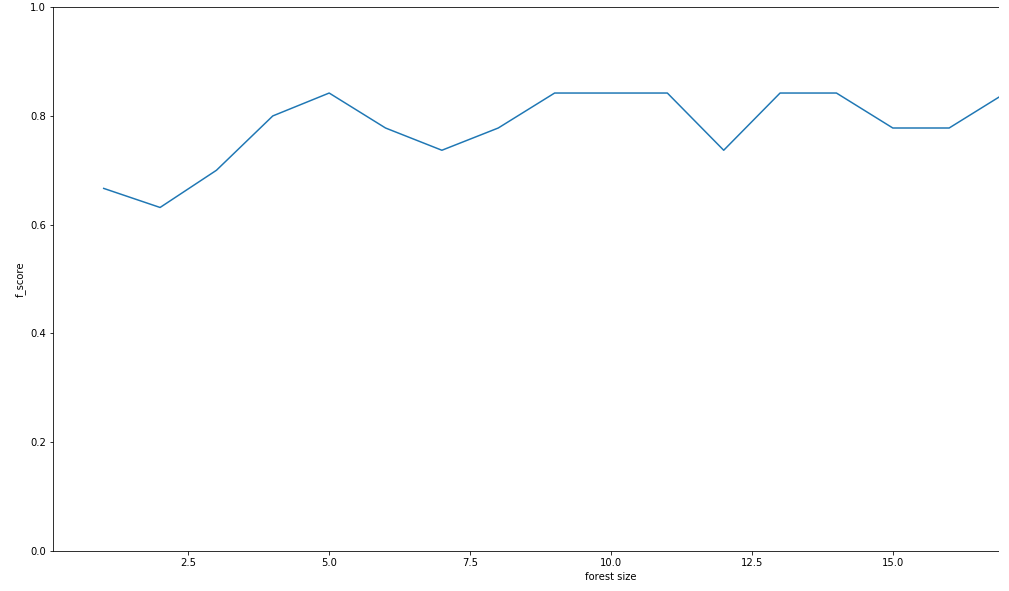
\includegraphics{images/forestsize.png}

\begin{center} Figure 4.1:Forest Size vs F1 Score \end{center}

According to the graph in Figure 4.1, the model performs the best at
about forest sizes greater than 5. Beyond this value, the graph shows
that there is no meaningful increase in the model's performance as the
forest size increases.

\subsubsection{Minimum Impurity Split}\label{minimum-impurity-split}

The model's minimum impurity parameter was also tuned. Minimum impurity
refers to the value in which the algorithm decides to split the tree
into subtrees. A conservative approach in building each tree in the
forest is making a tree split only when both subtrees are purely valid
bacteria and purely invalid bacteria. This approach is prone to
overfitting since it doesn't forgive impurities from outlier samples. By
setting the minimum impurity to a higher value, the algorithm becomes
more lenient in its tree splits, forgiving noise and outliers. Although,
if minimum impurity is set too high, the algorithm may be too lenient
that it may forgive even incorrect tree splits that do not actually
represent relationships in the data. Finding the best amount of impurity
is similar to finding the best forest size. The model is fit with
varying minimum impurities from impurity=0 to impurity=1.

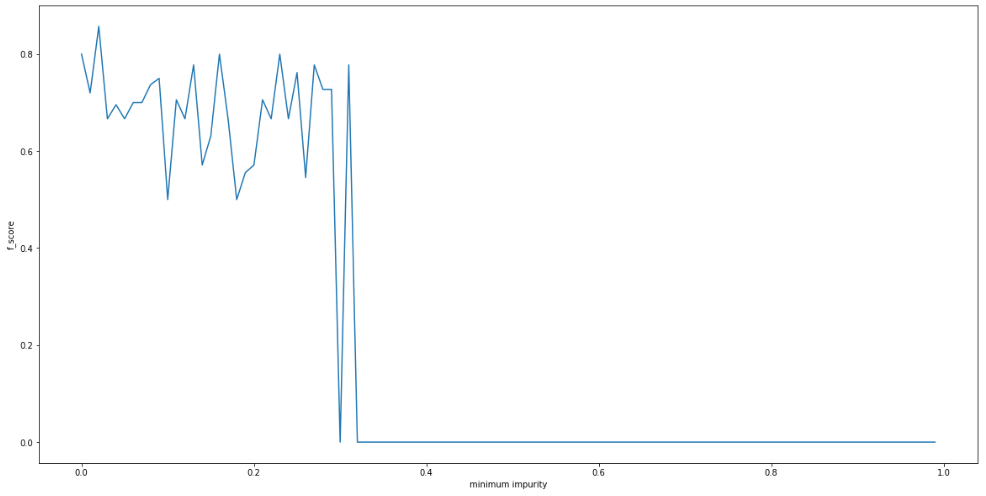
\includegraphics{images/impurity.png}

\begin{center} Figure 4.2:Minimum Impurity Threshold vs F1 Score \end{center}

The best performing minimum values of impurity are found between 0 to
0.1. According to the graph in Figure 4.2, the best performing minimum
values of impurity were found between 0 to 0.1. The model's performance
experiences higher variance beyond this value. As soon as impurity
exceeds 0.3, the performance drops to zero because splits become too
forgiving that the tree becomes meaningless.

\subsection{Artificial Neural
Network}\label{artificial-neural-network-1}

\subsubsection{Number of Nodes in 1 Hidden
Layer}\label{number-of-nodes-in-1-hidden-layer}

The number of nodes in the hidden layer of a neural network also affects
the model's performance. Just like hidden layer sizes, having too few
neurons may affect the ability of the network to model the relationships
of the data while having too much neurons may slow down training and
promote overfitting (Hagan et al., 1996). There are also architectural
rules of thumb for choosing the number of neurons per layer. According
to Hagan et. al, (2014) one should begin with more than enough neurons
from the start (somwhere between \(N_i\) and \(N_o\). In this study
different neuron sizes were tested, between n=10 until n=300.

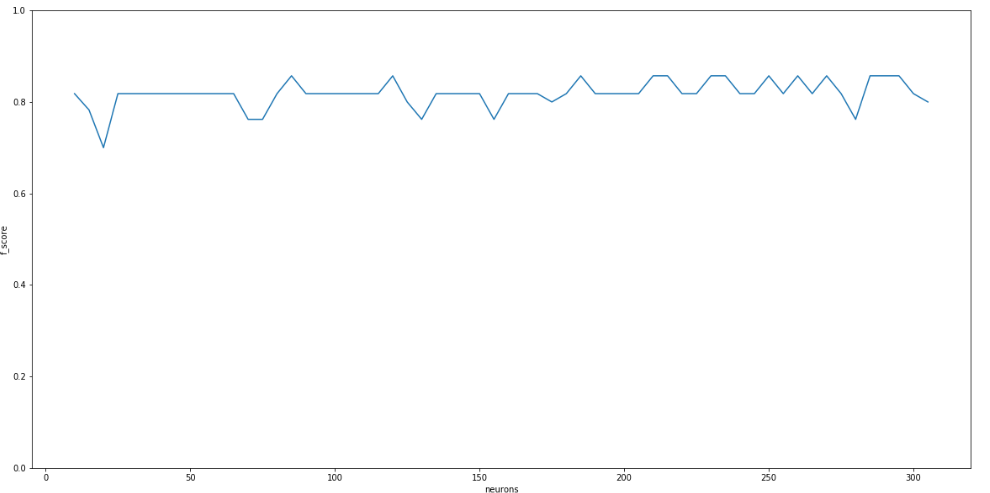
\includegraphics{images/neuronssize.png}

\begin{center} Figure 4.3:Number of Neurons vs F1 Score \end{center}

According to the graph in figure 4.3, the performance of the model is
fluctuates between 0.75 to 0.85 between n=10 and n=60. At about
n\textgreater{}60 the performance of the model stabilizes to a narrower
range, between 0.75 and 0.85. Increasing the number of neurons where 60
1\$. Despite knowing this, the model was still fit into different sizes
of hidden layers from n=1 to n=20 just for the purposes of testing.

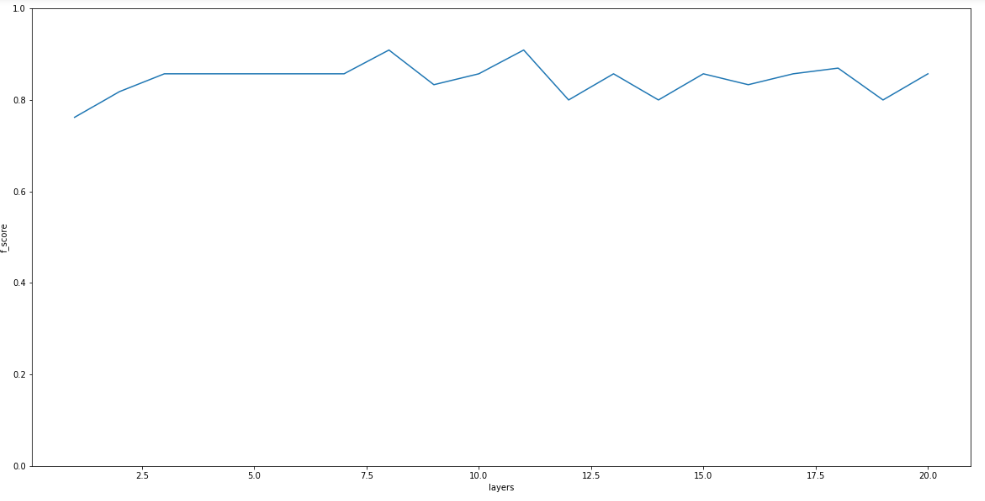
\includegraphics{images/layersize.png}

\begin{center} Figure 4.4:Hidden Layer Size vs F1 Score \end{center}

According to the graph in Figure 4.4, neural networks' performaces
fluctuate between 0.8 and 0.85. The size of the hidden layer does not
meaningfully affect this model's performance. After testing all this, it
was decided that the number of layers be set as small as possible (n=1)
to follow the architectural rule of thumb.

\section{Cross Validation}\label{cross-validation}

\subsection{F1 score as Performance
Measure}\label{f1-score-as-performance-measure}

The amount of positive (valid bacteria; n=195) and negative (invalid
bacteria;n=66) samples are unequal in this dataset. This means that
using the measure of accuracy:

\begin{equation} \mathrm{accuracy}=\frac{tP + tN}{N}  \end{equation}

where \(tP\) is the number of true positives (predicted positive and
actually positive); \(tN\) is the number of true negatives (predicted
negative and actually positive); and \(N\) is the total size of the test
partition.

Accuracy will not be a good measure of model performance. This is
because having more positive data will reward higher accuracy to models
that have high frequencies of positive predictions. Using accuracy as a
measure of performance will favor models that ``cheat'' by simply
predicting positive for any sample. To avoid models cheating, the
measure f-1 score is used instead of accuracy. \(F_1\) score is defined
as:

\begin{equation} F_1 =2 \frac{\mathrm{precision}\cdot \mathrm{recall}}{\mathrm{precision} + \mathrm{recall}}  \end{equation}

where precision is defined as\\

\begin{equation} \mathrm{precision} =\frac{tN}{tP+fP}  \end{equation}

and recall is defined as

\begin{equation} \mathrm{recall} =\frac{tN}{tP+fN}  \end{equation}

\(fN\) stands for false negatives (predicted negative but actually
positive) and \(fP\) stands for false positives (predicted positive but
actually negative) \(F_1\) score is a more robust performance measure
since it takes into account both precision and recall. Despite having
unequal amounts of positive and negative data, \(F_1\) score can
accurately measure model performance.

\subsection{Measuring overfitting}\label{measuring-overfitting}

It was discussed in the previous sections how unreliable it is to
measure a model's performance using the same data it was trained on.
Having high performance on the training partition does not necessarily
mean that the model has successfully described the relationships of
data. High performance on the training partition could also mean that
the model is highly overfit to the training data. This is why in this
section, training performance and testing performance for each model is
compared. The following graphs show the effect of changing the
proportion of the two partitions to each model's performance. Each model
performance is tested from training proportion of 0.1
(train\_samples=26) to training proportion 0.75 (train\_samples=196).
Whatever is left in the whole dataset is used as the test proportion.

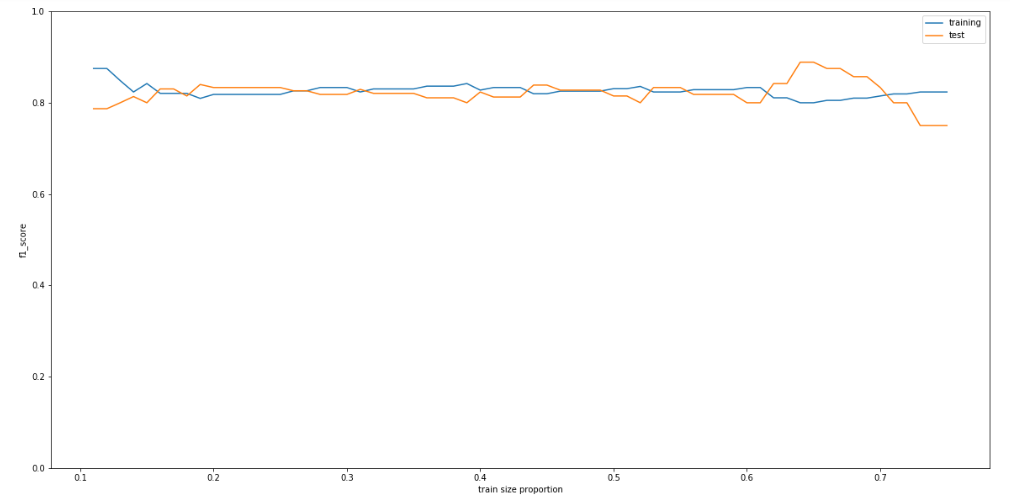
\includegraphics{images/bayesCV.png}

\begin{center} Figure 4.5:Naive Bayes Train Size Proportion vs F1 Score \end{center}

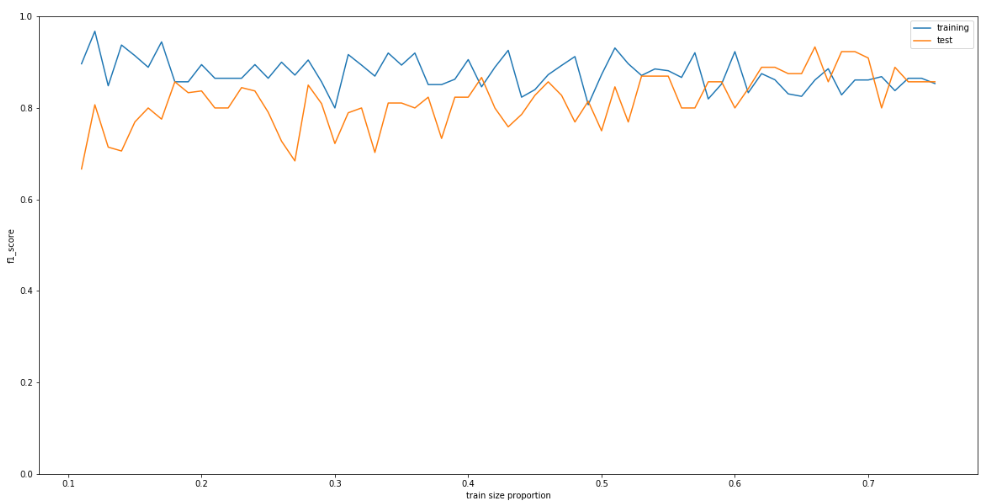
\includegraphics{images/treeCV.png}

\begin{center} Figure 4.6:Random Forest Classifier Train Size Proportion vs F1 Score \end{center}

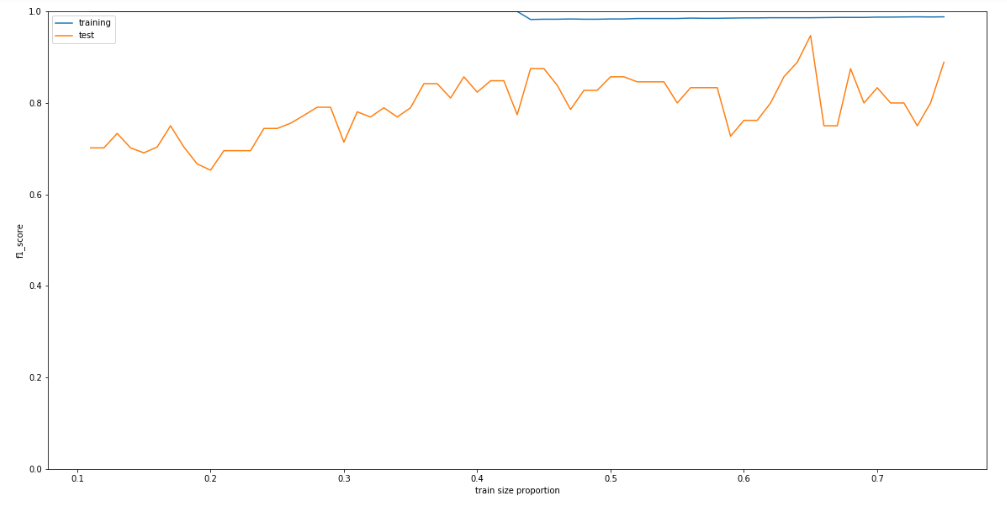
\includegraphics{images/nnCV.png}

\begin{center} Figure 4.7:Neural Network Train Size Proportion vs F1 Score \end{center}

All of the models show typical model behaviors. While the training
partition increases in size, training score decreases. This is because
more samples mean that noise and outliers are outscaled by the number of
samples, therefore, overfitting becomes less likely, decreasing the
performance on its own training data. On the other hand, while the
training partition increases in size, test score increases. This is
because the increase of training samples means that the model is able to
generalize the relationships easier. Good generalization is manifested
by a higher score in its test partition since this partition does not
share the noise and outlier samples of the training partition.

\chapter{Results}\label{results}

\section{Binarization of data}\label{binarization-of-data}

One of the observations this study makes is how the models perform
better when data is binarized. Instead of using each frequency value for
each gene (Cluster of Orthologous Genes), the model yielded higher cross
validation values when data was transformed through a binarization
function:

\begin{equation}
b(x) = \left\{\begin{matrix}
1 &{x>0} \\
0 & {x\leq 0}
\end{matrix}\right.
\end{equation}

This approach may work better because same COG's serve similar functions
(as discussed in a previous section in Chapter 2: Clusters of
Orthologous Genes). Using frequency distribution as data values may
obscure the relationships from the models due to the extra complexity.
It may also introduce more noise for the data making it highly prone to
overfitting.

\section{Minimum Set of Genes}\label{minimum-set-of-genes}

\subsection{Coefficient of likelihood for each
gene}\label{coefficient-of-likelihood-for-each-gene}

Using the Naive Bayes Classifier each a coefficient of likelihood for
each gene was obtained. The higher the coefficient of likelihood, the
higher the probability that this gene is part of the minimum set of
genes. The following graph in Figure 5.1 shows the frequency
distribution of gene likelihoods:

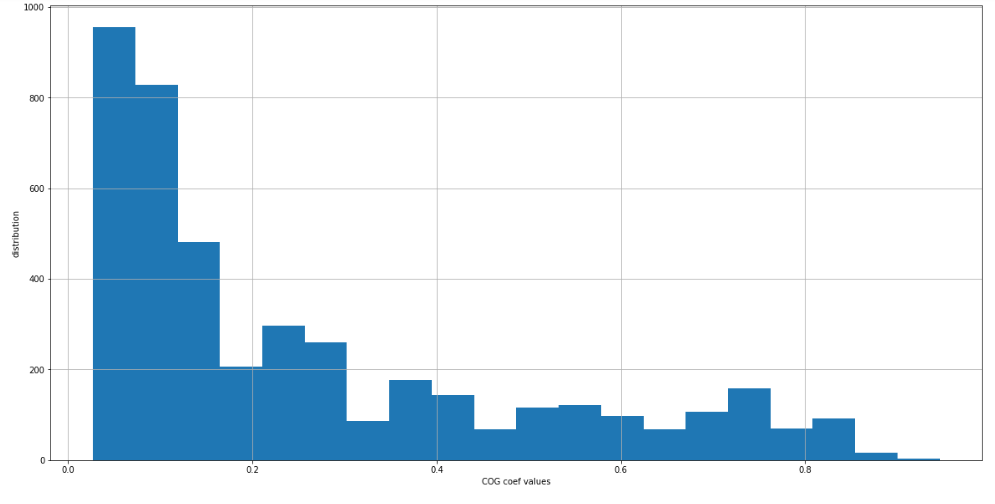
\includegraphics{./tex2pdf.9716/0ac99d6c6548095e4d165eb01da5a9dcc121c8fc.png}

\begin{center} Figure 5.1:Frequncy Distribution of coef Values vs F1 Score \end{center}

Figure 5.1 shows that the frequency of genes decreases as the
coefficient of likelihood increases. In fact there are only 3 genes with
coefficient of likelihood greater than or equal to 0.9. As we decrease
our coefficient of likelihood threshold, we can include more genes, as
seen in Table 5.1.

\begin{longtable}[]{@{}lr@{}}
\caption{Threshold of coefficient of likelihood and the corresponding
number of genes included in the set}\tabularnewline
\toprule
\begin{minipage}[b]{0.48\columnwidth}\raggedright\strut
\strut
\end{minipage} & \begin{minipage}[b]{0.48\columnwidth}\raggedleft\strut
Number of genes in the set\strut
\end{minipage}\tabularnewline
\midrule
\endfirsthead
\toprule
\begin{minipage}[b]{0.48\columnwidth}\raggedright\strut
\strut
\end{minipage} & \begin{minipage}[b]{0.48\columnwidth}\raggedleft\strut
Number of genes in the set\strut
\end{minipage}\tabularnewline
\midrule
\endhead
bayesian findings t=0.9 & 3\tabularnewline
bayesian findings t=0.8 & 110\tabularnewline
bayesian findings t=0.7 & 393\tabularnewline
bayesian findings t=0.6 & 566\tabularnewline
\bottomrule
\end{longtable}

\subsection{Decision trees of important
genes}\label{decision-trees-of-important-genes}

Using the Random forest classifier, 5 decision trees were obtained.
These trees model the relationship of genes to bacterial validity.

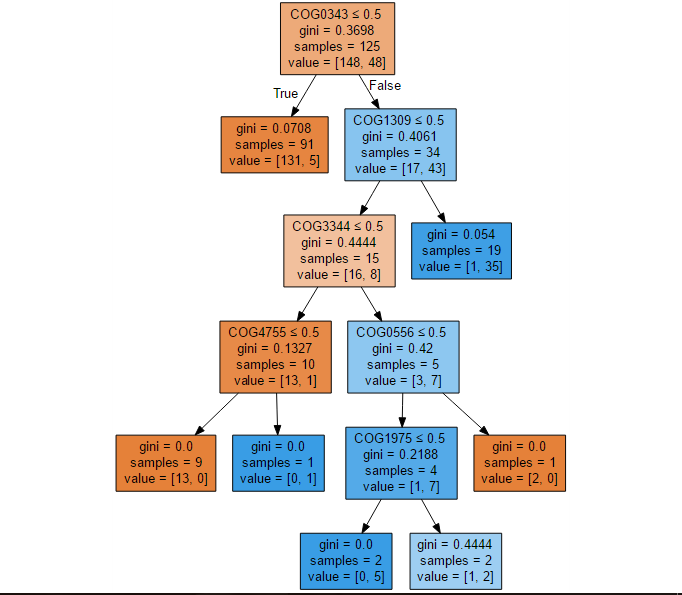
\includegraphics{images/tree1.PNG}

\begin{center} Figure 5.2: One of the 5 trees in the forest \end{center}

Genes which are closer to the root nodes are genes which are more likely
part of the minimum set of genes since these genes are the primary
splitters between valid and invalid bacteria. This means that the
presence or absence of these genes describe the difference between each
valid and invalid bacteria. Genes located farther from the root node are
genes that may exhibit conditional essentiality from its parent genes.

\subsection{Matrix of network weights}\label{matrix-of-network-weights}

Using the artificial neural network 2 matrices of interconnection
weights were obtained. Since the architecture of the neural network is
4346-75-1 (4356 features/input neurons, 75 hidden layer neurons, 1
output class) the two matrices are o sizes \(W_1:4346 \times 75\) and
\(W_2:75 \times 1\). We can infer which neurons in the hidden layers
classify for valid bacteria by looking at matrix \(W_2\). Highly
positive values in \(W_2\) indicate neurons that are strong determinants
of bacterial validity. Each of these hidden layer neurons have a
corresponding column in matrix \(W_1\).

Therefore the gene weights (weights of interconnections between input
and hidden layer) of highly positive hidden neurons with higher values
will correspond genes which are more likely part of the minimum set of
genes.

\chapter{Discussions}\label{discussions}

Each of the models were able to model the relationships with relatively
high performance (Naive Bayes f1\_score=0.80; Random Forest Classifier
f1\_score=0.78; Artificial Neural Network f1\_score=0.87) but the main
focus of the study was each of the model's representation of the minimum
set of genes. In the representation aspect, each of the model's show its
own respective advantages and disadvantages. The Random Forest
Classifier was able to show complex conditional relationships of genes
with each other but this models feature's cannot be represented as a set
of genes. It was the Naive Bayes Classifier which was able to represent
its features as coefficient of likelihoods that correspond to each
gene's likelihood of being an element of the minimum set of genes.

\section{Comparing findings to an existing
database}\label{comparing-findings-to-an-existing-database}

By obtaining the important features on each model, this study was able
to propose its own findings on the concept of minimum gene set. Using
the CEG database as a point of comparison, the following results were
obtained:

\begin{longtable}[]{@{}lrr@{}}
\caption{Jaccard index values of each model and their corresponding
feature importance threshold (t)}\tabularnewline
\toprule
\begin{minipage}[b]{0.32\columnwidth}\raggedright\strut
\strut
\end{minipage} & \begin{minipage}[b]{0.32\columnwidth}\raggedleft\strut
CEG essential genes\strut
\end{minipage} & \begin{minipage}[b]{0.32\columnwidth}\raggedleft\strut
non essential genes\strut
\end{minipage}\tabularnewline
\midrule
\endfirsthead
\toprule
\begin{minipage}[b]{0.32\columnwidth}\raggedright\strut
\strut
\end{minipage} & \begin{minipage}[b]{0.32\columnwidth}\raggedleft\strut
CEG essential genes\strut
\end{minipage} & \begin{minipage}[b]{0.32\columnwidth}\raggedleft\strut
non essential genes\strut
\end{minipage}\tabularnewline
\midrule
\endhead
bayesian findings t=0.9 & 0.00149775 & 0\tabularnewline
bayesian findings t=0.8 & 0.0549176 & 0\tabularnewline
bayesian findings t=0.7 & 0.191447 & 0.00245776\tabularnewline
bayesian findings t=0.6 & 0.269896 & 0.0058548\tabularnewline
nn findings t=0.9 & 0.0684466 & 0.0189306\tabularnewline
nn findings t=0.8 & 0.130047 & 0.0403559\tabularnewline
nn findings t=0.7 & 0.189569 & 0.0614355\tabularnewline
nn findings t=0.6 & 0.23507 & 0.104526\tabularnewline
\bottomrule
\end{longtable}

Note that only the non-tree based models are in this table since the
random forest model's representation of the minimum set of genes cannot
be perfectly represented by feature importances. Random Forest
classifier represents feature importances as if-else conditional
relationships instead of individual weighted coefficients for each gene.
Table 5.2 shows the Jaccard index of each model's obtained gene set and
the CEG databases gene set. Jaccard index \(\mathrm{J(A,B)}\) is a
measure used to compare similarity over two sets. Jaccard index is
defined by:

\begin{equation} \mathrm{J(A,B)}=\frac{|\mathrm{A} \cap \mathrm{B}|}{|\mathrm{A} \cup \mathrm{B}|}  \end{equation}

Table 5.2 shows that the gene sets obtained by this study are smaller
than the gene set in the CEG database. There could be two reasons behind
this disparity in gene sets.

\begin{enumerate}
\def\labelenumi{(\arabic{enumi})}
\item
  CEG database contain functionally redundant genes. The gene set
  obtained from the CEG database doesn't necessarily represent the
  minimum gene set itself, this gene set is merely the set of genes that
  have been defined as essential. There may be redundant functions in
  the CEG database itself which means that constructing a valid
  bacterium doesn't require exactly one of each gene defined in the
  database.
\item
  The model is unable to represent the minimum set of genes. Although
  the models yield high scores in classifying between valid and invalid
  bacteria, this doesn't mean that models are able to perfectly
  represent the minimum set of genes. This could be the consequence if
  the data used in training isn't enough to represent the whole
  population of valid and invalid bacteria. There may be samples of
  bacteria that are not represented in any of the samples in the data.
  If this is truly the case the model would be unaware of relationships
  of genes and validity of these underrepresented bacteria. Although all
  of the models genes sets are similar in the sense that all are smaller
  than the CEG database, the two models differ in their ability to
  determine nonessential genes. The Bayesian classifier's Jaccard index
  when compared to the non-essential gene set is smaller than the neural
  network classifiers Jaccard Index. This means that the neural network
  classifier has more genes misidentified as essential. This is a
  surprising result given that the neural network slightly outperforms
  the Bayesian classifier. The neural network's classifier's poor
  performance in identifying non-essential genes could be attributed to
  its own model representation of the minimum set of genes. It was
  discussed earlier how neural network classifiers are black box models.
  Even though these type of models perform well in classification, they
  are not widely used in feature analyses of data because of their
  complex and black boxed structure.
\end{enumerate}

\chapter{Conclusion}\label{conclusion}

The advent of big data and machine learning has contributed to the
growth of many fields. In this study, machine learning was used in the
field of genomics and bioinformatics, particularly on the concept of the
minimum set of genes. Multiple machine learning algorithms (Naive Bayes,
Random Forest, Artificial Neural Network) were used to model the
relationship between bacterial validity and genes. Training using data
from COG annotated gene sequences, the models were able to classify the
validity of a given bacterium based only on its genes. The models show
promising predictive power (Naive Bayes Classifier=0.80, Random Forest
Classifier=0.78, and Artificial Neural Network=0.87). Each model is then
subjected to feature extraction to describe a its own interpretation of
the minimum set of genes. Each of the models' set of genes are compared
the CEG databases set of essential genes. The results show that even
though the Naive Bayes Classifier does not have the most predictive
power, it is able to perform best in the set comparisons between the CEG
database. In particular it was the best model in classifying which genes
are non-essential (Jaccard index of 0.0058 when compared to CEG set of
nonessential genes)

As a recommendation, future studies could focus on selecting more robust
methods in extracting feature importance. This especially applies to the
extraction of feature importance in a neural network model. At the time
of writing this paper, there is still no widespread consensus as to
which feature extraction method is best in neural network models. In the
future when there is one, the study of minimum set of genes will surely
benefit from it. It is also advisable for future studies to include
other families of classifiers like SVM, KNN or maybe unsupervised
algorithms like K means clustering.

In conclusion, this study answers the research question formulated in
chapter 3: ``Are these machine learning classifiers a valid tool for
determining the minimal set of genes?''. After considering the results
of each machine learning algorithm, the hypothesis discussed from
chapter 3 is accepted. The study shows that there is good promise in the
application of machine learning in the study of the minimum set of
genes. The study on the minimum set of genes has been an open problem
ever since the emergence of the field of genomics. This study is the
first of kind in the sense that this was the first attempt in applying
machine learning algorithms to model the minimum set of genes. Research
on the field of bio-informatics and machine learning are still emerging,
in the future when data is more abundant and tools are more advanced,
this study would be a good framework for more large-scale and in depth
studies.

\chapter*{References}\label{references}
\addcontentsline{toc}{chapter}{References}

\hypertarget{refs}{}
\hypertarget{ref-Akerley1998}{}
Akerley, B. J., Rubin, E. J., Camilli, A., Lampe, D. J., Robertson, H.
M., \& Mekalanos, J. J. (1998). Systematic identification of essential
genes by in vitro mariner mutagenesis. \emph{Proceedings of the National
Academy of Sciences}, \emph{95}(15), 8927--8932.
\url{http://doi.org/10.1073/pnas.95.15.8927}

\hypertarget{ref-Benson2000a}{}
Benson, D. A., Karsch-Mizrachi, I., Lipman, D. J., Ostell, J., Rapp, B.
A., \& Wheeler, D. L. (2000). GenBank. \emph{Nucleic Acids Research},
\emph{28}(1), 15--8. \url{http://doi.org/10.1093/nar/28.1.15}

\hypertarget{ref-DeBerardinis2008}{}
Berardinis, V. de, Vallenet, D., Castelli, V., Besnard, M., Pinet, A.,
Cruaud, C., \ldots{} Weissenbach, J. (2008). A complete collection of
single-gene deletion mutants of Acinetobacter baylyi ADP1.
\emph{Molecular Systems Biology}, \emph{4}, 174.
\url{http://doi.org/10.1038/msb.2008.10}

\hypertarget{ref-Crick1958}{}
Crick, F. H. (1958). On protein synthesis. \emph{Symposia of the Society
for Experimental Biology}, \emph{12}, 138--163.
\url{http://doi.org/10.1038/227561a0}

\hypertarget{ref-Dietterich2000}{}
Dietterich, T. G. (2000). An Experimental Comparison of Three Methods
for Constructing Ensembles of Decision Trees. \emph{Machine Learning},
\emph{40}(2), 139--157. \url{http://doi.org/10.1023/A:1007607513941}

\hypertarget{ref-DiazUriarte2006}{}
Díaz-Uriarte, R., \& Alvarez de Andrés, S. (2006). Gene selection and
classification of microarray data using random forest. \emph{BMC
Bioinformatics}, \emph{7}(6), 3.
\url{http://doi.org/10.1186/1471-2105-7-3}

\hypertarget{ref-Ferber2004}{}
Ferber, D. (2004). SYNTHETIC BIOLOGY: Microbes Made to Order.
\emph{Science}, \emph{303}(5655), 158--161.
\url{http://doi.org/10.1126/science.303.5655.158}

\hypertarget{ref-Fleischmann1995}{}
Fleischmann, R., Adams, M., White, O., Clayton, R., Kirkness, E.,
Kerlavage, A., \ldots{} Al., E. (1995). Whole-genome random sequencing
and assembly of Haemophilus influenzae Rd. \emph{Science},
\emph{269}(5223), 496--512. \url{http://doi.org/10.1126/science.7542800}

\hypertarget{ref-Fraser1995}{}
Fraser, C. M., Gocayne, J. D., White, O., Adams, M. D., Clayton, R. A.,
Fleischmann, R. D., \ldots{} Venter, J. C. (1995). The Minimal Gene
Complement of Mycoplasma genitalium. \emph{Science}, \emph{270}(5235),
397--403. \url{http://doi.org/10.1126/science.270.5235.397}

\hypertarget{ref-Galperin2015}{}
Galperin, M. Y., Makarova, K. S., Wolf, Y. I., \& Koonin, E. V. (2015).
Expanded Microbial genome coverage and improved protein family
annotation in the COG database. \emph{Nucleic Acids Research},
\emph{43}(D1), D261--D269. \url{http://doi.org/10.1093/nar/gku1223}

\hypertarget{ref-Gerdes2006}{}
Gerdes, S., Edwards, R., Kubal, M., Fonstein, M., Stevens, R., \&
Osterman, A. (2006). Essential genes on metabolic maps. \emph{Current
Opinion in Biotechnology}, \emph{17}(5), 448--456.
\url{http://doi.org/10.1016/j.copbio.2006.08.006}

\hypertarget{ref-Glass2006}{}
Glass, J. I., Assad-Garcia, N., Alperovich, N., Yooseph, S., Lewis, M.
R., Maruf, M., \ldots{} Venter, J. C. (2006). Essential genes of a
minimal bacterium. \emph{Proceedings of the National Academy of Sciences
of the United States of America}, \emph{103}(2), 425--30.
\url{http://doi.org/10.1073/pnas.0510013103}

\hypertarget{ref-Hagan1996}{}
Hagan, M. T., Demuch, H. B., \& Beale, M. (1996). \emph{Neural Network
Design} (p. 732). {[}publisher not identified{]}. Retrieved from
\url{http://hagan.okstate.edu/nnd.html}

\hypertarget{ref-Hamer2001}{}
Hamer, L., DeZwaan, T. M., Montenegro-Chamorro, M. V., Frank, S. A., \&
Hamer, J. E. (2001). Recent advances in large-scale transposon
mutagenesis. \emph{Current Opinion in Chemical Biology}, \emph{5}(1),
67--73. \url{http://doi.org/10.1016/S1367-5931(00)00162-9}

\hypertarget{ref-HutchisonIII1999}{}
Hutchison III, C. A. (1999). Global transposon mutagenesis and a minimal
Mycoplasma genome. \emph{Science}, \emph{286}(5447), 2165--2169.
\url{http://doi.org/10.1126/science.286.5447.2165}

\hypertarget{ref-Kobayashi2003}{}
Kobayashi, K., Ehrlich, S. D., Albertini, A., Amati, G., Andersen, K.
K., Arnaud, M., \ldots{} Ogasawara, N. (2003). Essential Bacillus
subtilis genes. \emph{Proceedings of the National Academy of Sciences},
\emph{100}(8), 4678--4683. \url{http://doi.org/10.1073/pnas.0730515100}

\hypertarget{ref-Koonin2000}{}
Koonin, E. V. (2000). How many genes can make a cell: The Minimal-Gene
Set Concept. \emph{Annual Review of Genomics Human Genetics},
\emph{1}(1), 99--116. \url{http://doi.org/10.1146/annurev.genom.1.1.99}

\hypertarget{ref-Leavitt2010}{}
Leavitt, S. A. (2010). Deciphering the Genetic Code: Marshall Nirenberg.
\emph{Office of NIH History}. Retrieved from
\url{https://history.nih.gov/exhibits/nirenberg/glossary.htm}

\hypertarget{ref-Leinonen2011}{}
Leinonen, R., Akhtar, R., Birney, E., Bower, L., Cerdeno-T??rraga, A.,
Cheng, Y., \ldots{} Cochrane, G. (2011). The European nucleotide
archive. \emph{Nucleic Acids Research}, \emph{39}(SUPPL. 1), D28--D31.
\url{http://doi.org/10.1093/nar/gkq967}

\hypertarget{ref-Leinonen2011a}{}
Leinonen, R., Sugawara, H., \& Shumway, M. (2011). The sequence read
archive. \emph{Nucleic Acids Research}, \emph{39}(SUPPL. 1), D19--D21.
\url{http://doi.org/10.1093/nar/gkq1019}

\hypertarget{ref-Lluch-Senar2015}{}
Lluch-Senar, M., Delgado, J., Chen, W.-H., Llorens-Rico, V., O'Reilly,
F. J., Wodke, J. A., \ldots{} Serrano, L. (2015). Defining a minimal
cell: essentiality of small ORFs and ncRNAs in a genome-reduced
bacterium. \emph{Molecular Systems Biology}, \emph{11}(1), 780--780.
\url{http://doi.org/10.15252/msb.20145558}

\hypertarget{ref-Mori2015}{}
Mori, H., Baba, T., Yokoyama, K., Takeuchi, R., Nomura, W., Makishi, K.,
\ldots{} Wanner, B. L. (2015). \emph{Identification of essential genes
and synthetic lethal gene combinations in Escherichia coli K-12.} (Vol.
1279, pp. 45--65). \url{http://doi.org/10.1007/978-1-4939-2398-4_4}

\hypertarget{ref-Mushegian1996}{}
Mushegian, A. R., \& Koonin, E. V. (1996). A minimal gene set for
cellular life derived by comparison of complete bacterial genomes.
\emph{Proceedings of the National Academy of Sciences}, \emph{93}(19),
10268--10273. \url{http://doi.org/10.1073/pnas.93.19.10268}

\hypertarget{ref-Nowak1997}{}
Nowak, M. A., Boerlijst, M. C., Cooke, J., \& Maynard Smith, J. (1997).
Evolution of genetic redundancy. \emph{Nature}, \emph{388}(6638),
167--71. \url{http://doi.org/10.1038/40618}

\hypertarget{ref-Pal2006}{}
Pál, C., Papp, B., Lercher, M. J., Csermely, P., Oliver, S. G., \&
Hurst, L. D. (2006). Chance and necessity in the evolution of minimal
metabolic networks. \emph{Nature}, \emph{440}(7084), 667--670.
\url{http://doi.org/10.1038/nature04568}

\hypertarget{ref-Smith2014}{}
Smith, M. K. (2014). Overfitting. Retrieved from
\url{http://www.ma.utexas.edu/users/mks/statmistakes/ovefitting.html}

\hypertarget{ref-Steinberg2014}{}
Steinberg, D. (2014). Why Data Scientists Split Data into Train and
Test. Retrieved from
\url{http://info.salford-systems.com/blog/bid/337783/Why-Data-Scientists-Split-Data-into-Train-and-Test}

\hypertarget{ref-Tatusov1997}{}
Tatusov, R. L. (1997). A Genomic Perspective on Protein Families.
\emph{Science}, \emph{278}(5338), 631--637.
\url{http://doi.org/10.1126/science.278.5338.631}

\hypertarget{ref-Tettelin2005}{}
Tettelin, H., Masignani, V., Cieslewicz, M. J., Donati, C., Medini, D.,
Ward, N. L., \ldots{} Fraser, C. M. (2005). Genome analysis of multiple
pathogenic isolates of Streptococcus agalactiae: Implications for the
microbial ``pan-genome''. \emph{Proceedings of the National Academy of
Sciences}, \emph{102}(39), 13950--13955.
\url{http://doi.org/10.1073/pnas.0506758102}

\hypertarget{ref-Tettelin2008}{}
Tettelin, H., Riley, D., Cattuto, C., \& Medini, D. (2008). Comparative
genomics: the bacterial pan-genome.
\url{http://doi.org/10.1016/j.mib.2008.09.006}

\hypertarget{ref-Thanassi2002}{}
Thanassi, J. A. (2002). Identification of 113 conserved essential genes
using a high-throughput gene disruption system in Streptococcus
pneumoniae. \emph{Nucleic Acids Research}, \emph{30}(14), 3152--3162.
\url{http://doi.org/10.1093/nar/gkf418}

\hypertarget{ref-VanTonder2014}{}
Tonder, A. J. van, Mistry, S., Bray, J. E., Hill, D. M. C., Cody, A. J.,
Farmer, C. L., \ldots{} Brueggemann, A. B. (2014). Defining the
Estimated Core Genome of Bacterial Populations Using a Bayesian Decision
Model. \emph{PLoS Computational Biology}, \emph{10}(8), e1003788.
\url{http://doi.org/10.1371/journal.pcbi.1003788}

\hypertarget{ref-Tripp2011}{}
Tripp, S., \& Grueber, M. (2011). Economic Impact of the Human Genome
Project. \url{http://doi.org/10.1017/CBO9781107415324.004}

\hypertarget{ref-Zhang2004}{}
Zhang, H. (2004). The Optimality of Naive Bayes. \emph{Proceedings of
the Seventeenth International Florida Artificial Intelligence Research
Society Conference FLAIRS 2004}, \emph{1}(2), 1--6.
\url{http://doi.org/10.1016/j.patrec.2005.12.001}

\hypertarget{ref-Zhang2009}{}
Zhang, R., \& Lin, Y. (2009). DEG 5.0, a database of essential genes in
both prokaryotes and eukaryotes. \emph{Nucleic Acids Research},
\emph{37}(SUPPL. 1), D455--8. \url{http://doi.org/10.1093/nar/gkn858}


\printbibliography



\end{document}
